\section{Calibration}

The calibration of the LTCC detector consisted of matching the gains of the 216 PMTs.
The main reason for this is that the FADC250 threshold parameters the same for all PMT.

This was accomplished by using normal production dataset.
A random trigger was saved in the datastream using a prescale factor of 100. This is ideal to select
events with the PMT noise, containing the Single Photo-electron signal.  





\begin{figure}
	\centering
	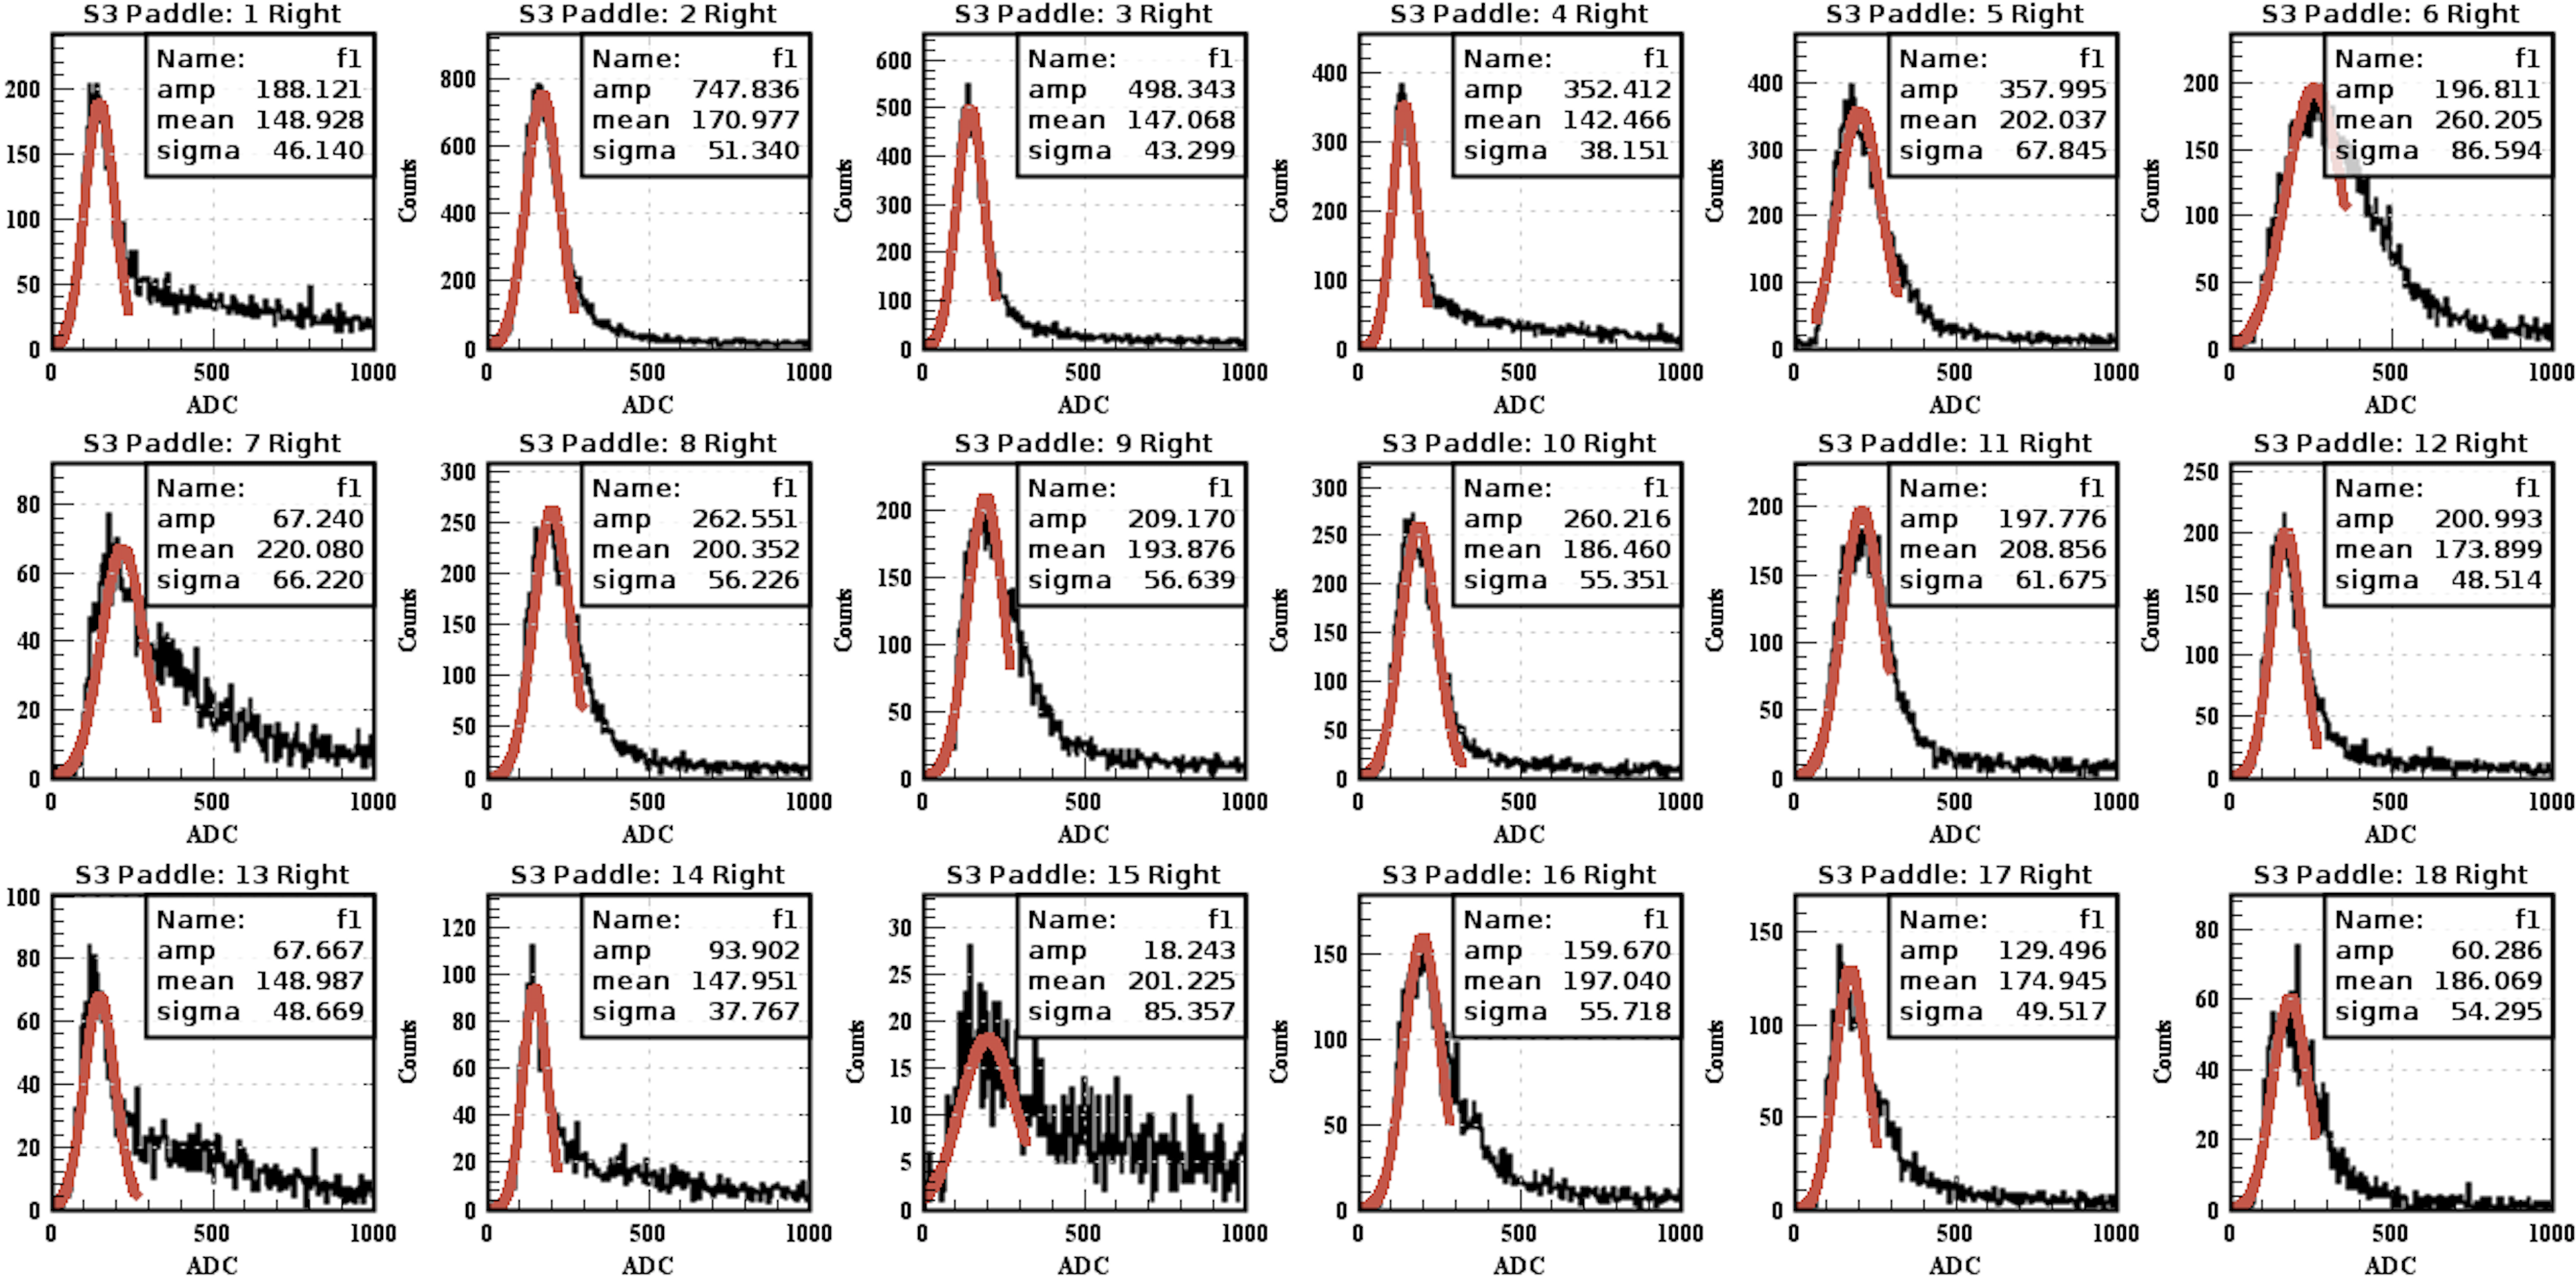
\includegraphics[width=0.95\columnwidth,keepaspectratio]{img/spe.png}
	\caption{The electronic scheme of the LTCC.}
	\label{fig:speCalibration}
\end{figure}


\paragraph{PMT gain matching}


\begin{figure}
	\centering
	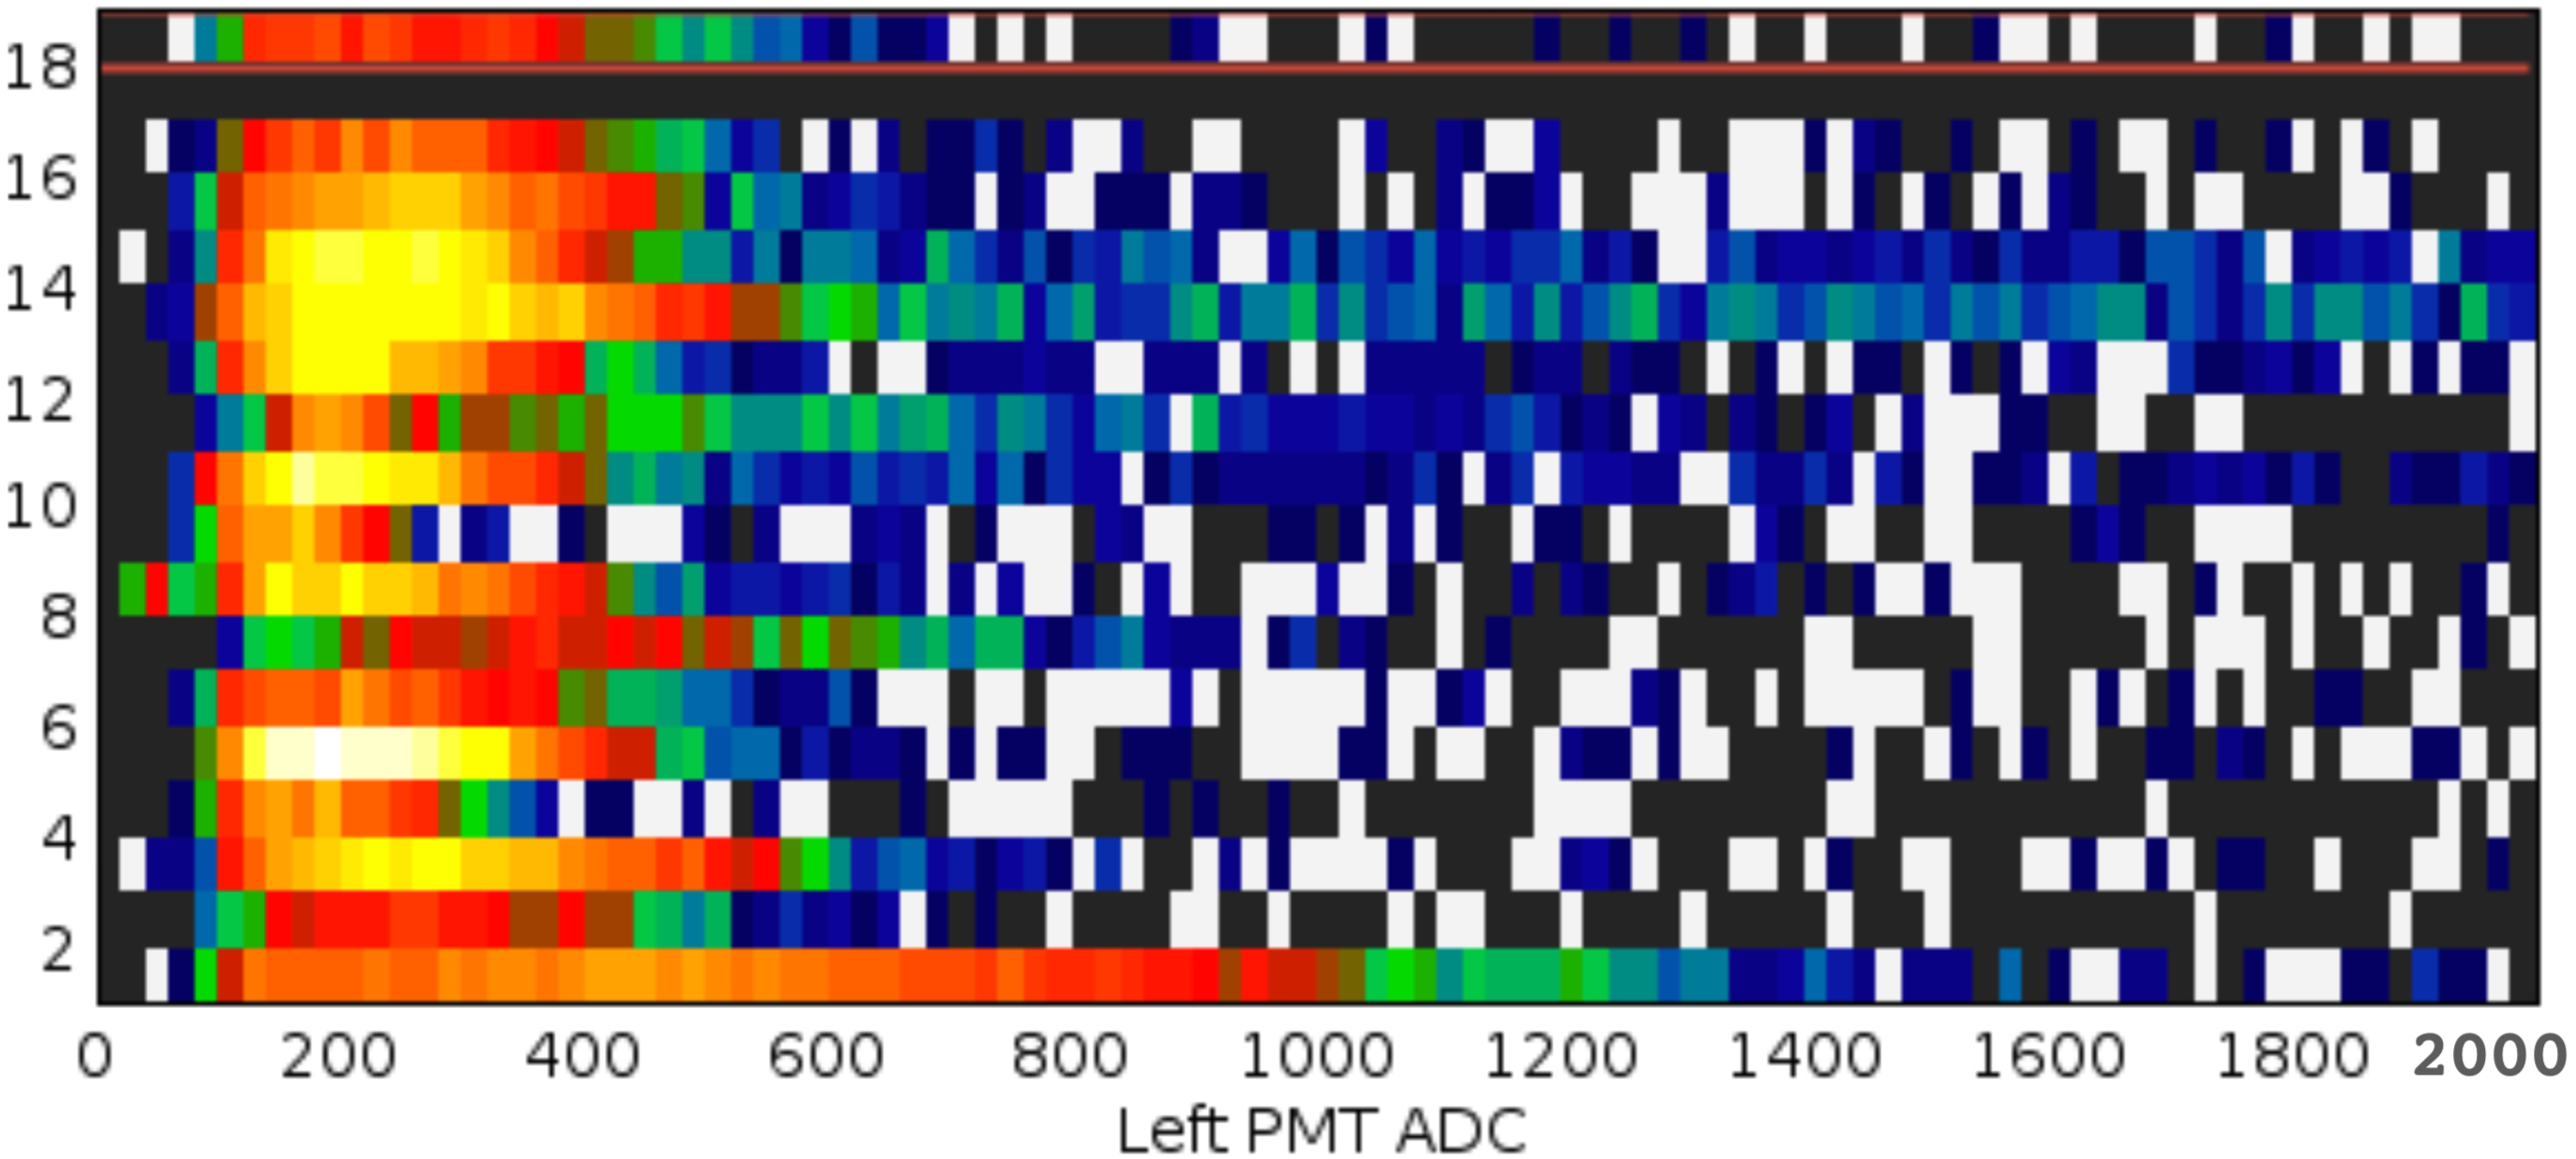
\includegraphics[width=0.95\columnwidth,keepaspectratio]{img/gainMatchingBefore.png}
	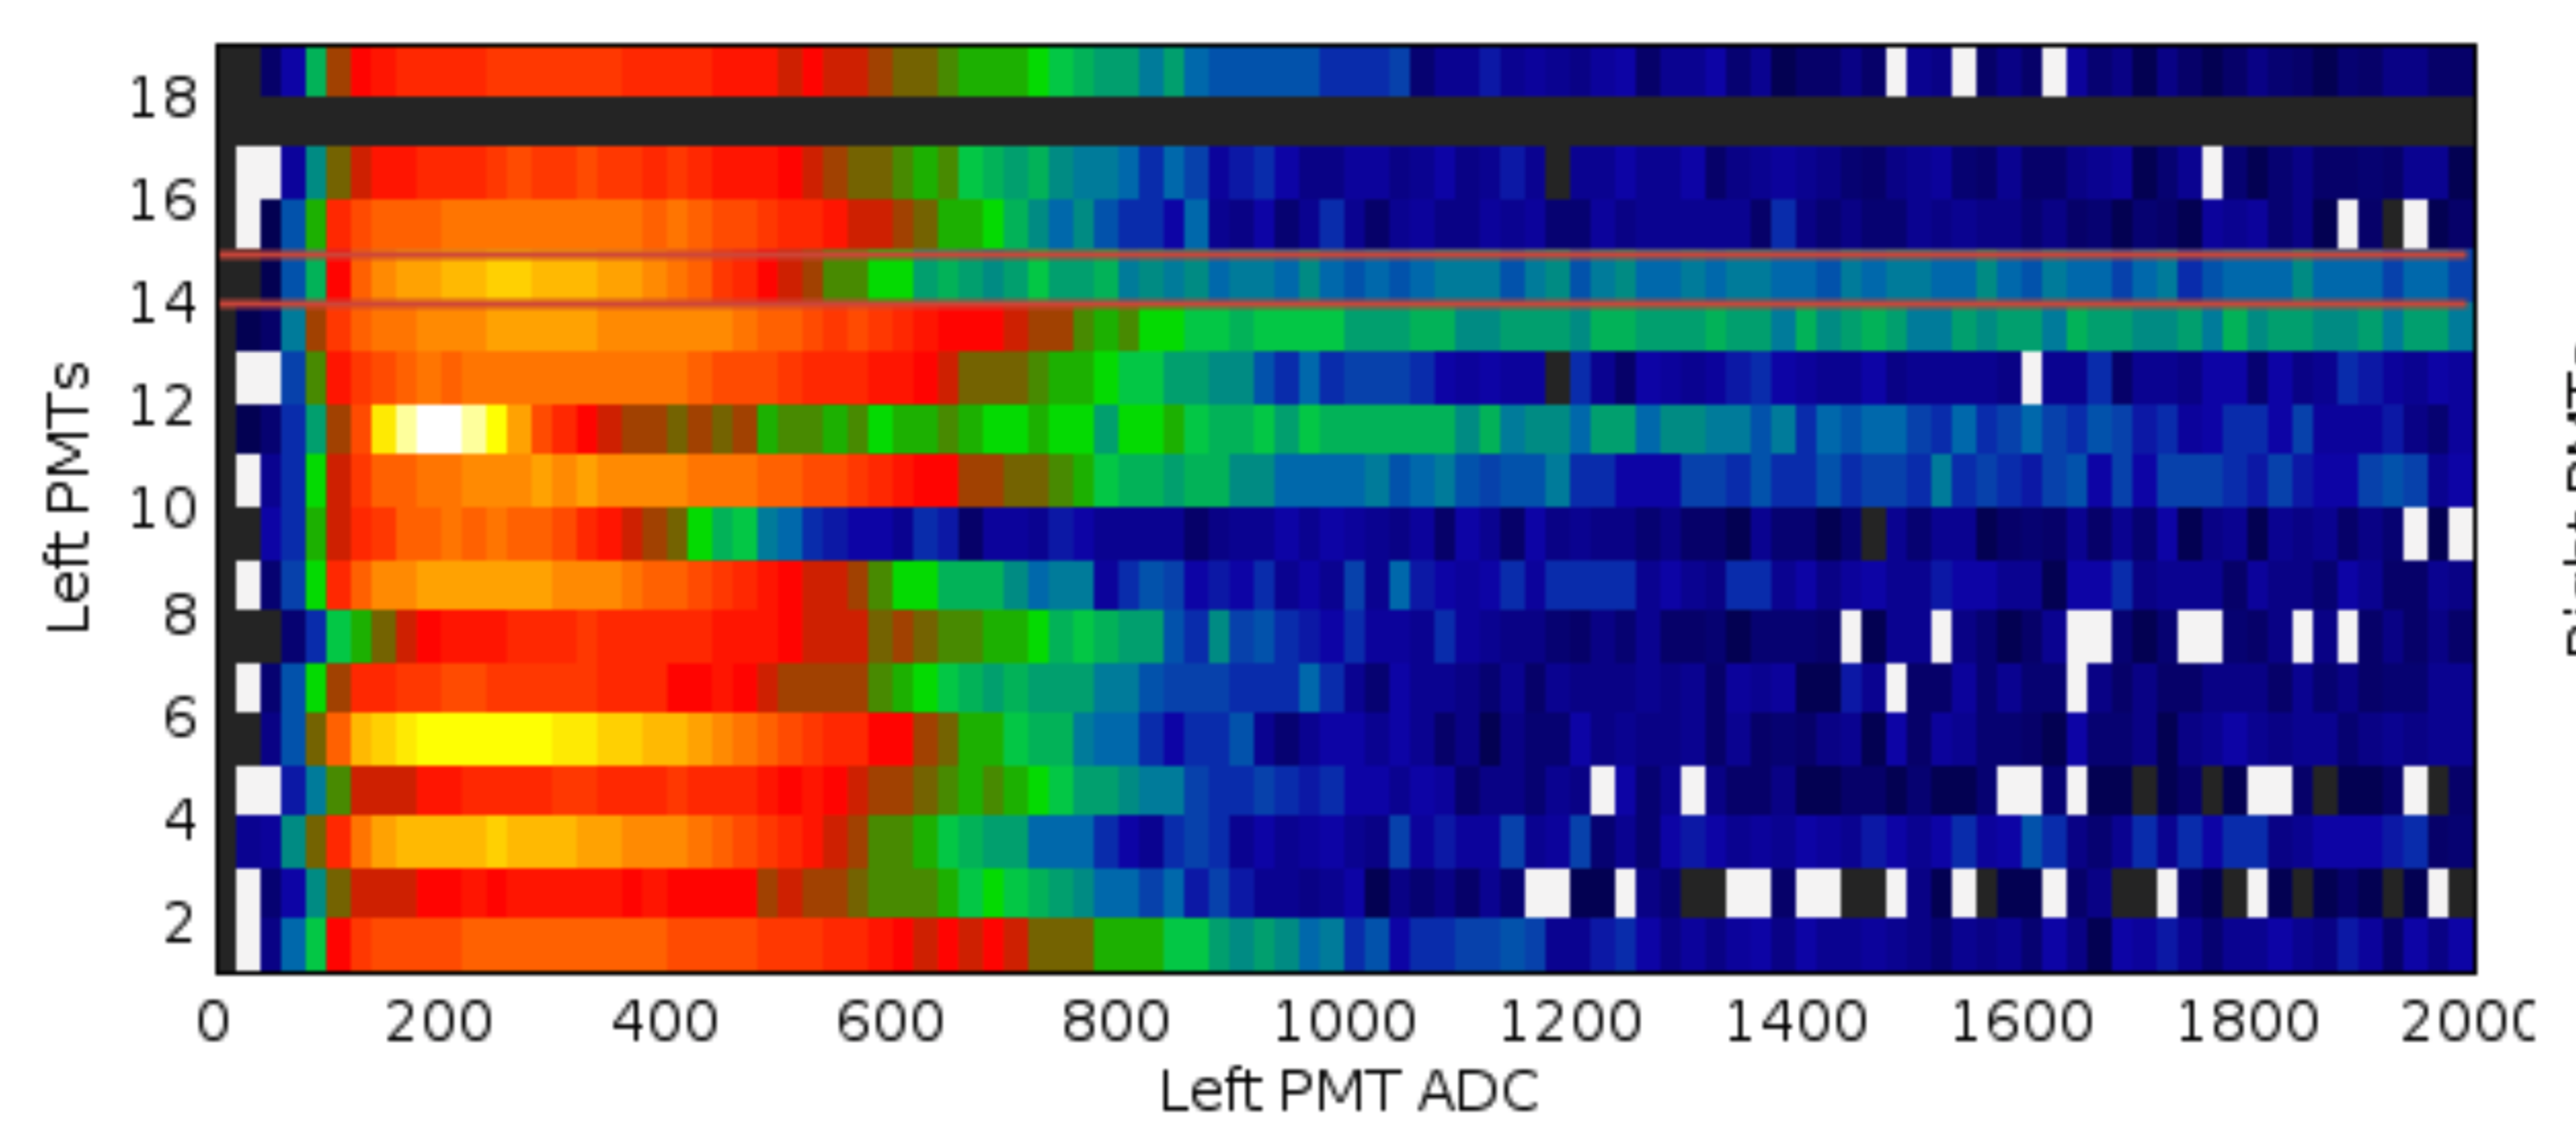
\includegraphics[width=0.95\columnwidth,keepaspectratio]{img/gainMatchingAfter.png}
	\caption{The electronic scheme of the LTCC.}
	\label{fig:gainMatching}
\end{figure}




